\section{Related Work}
\subsection{Parallel Real-time Job}
\begin{frame}
  \frametitle{Related Work --- Parallel Real-time Job}
  \begin{itemize}
    \item Reliability-Driven method by Qin et al.
      \footnote[frame]{\tiny\fullcite{cite:qin-reliability-driven}}
    \item He et al. viewed it as hybrid of periodic and aperiodic jobs
      and proposed a method by modeling spare capabilities
      \footnote[frame]{\tiny\fullcite{cite:he-spare-capabilities}}
    \item TAPADS by Xie et al. with deadline and security constraints.
      \footnote[frame]{\tiny\fullcite{cite:roystonea}}
  \end{itemize}
\end{frame}
\subsection{SLA Jobs}
\begin{frame}
  \frametitle{Related Work --- Scheduling with SLAs}
  User utility based:
  \begin{itemize}
    \item Libra --- computational economy driven scheduling
      \footnote[frame]{\tiny\fullcite{cite:libra}}
    \item Yeo et al. proposed a framework with linear penalty model on
      user utility.
      \footnote[frame]{\tiny\fullcite{cite:yeo-SLA-penalty}}
  \end{itemize}
  Grid computing
  \begin{itemize}
    \item He et al. proposed a two level optimization --- MUSCLE, a
      multi-cluster level scheduler, and TITAN, a single-cluster level
      workload manager.
      \footnote[frame]{\tiny\fullcite{cite:he-muscle-titan}}
  \end{itemize}
\end{frame}
\subsection{JPPF}
\begin{frame}
  \frametitle{Related Work --- JPPF}
  \begin{columns}
    \begin{column}{.6\textwidth}
      \begin{itemize}
        \item A popular open-source cluster management framework.
        \item Easy to deploy.
        \item Provides an easy to use GUI management tool.
        \item Abundant APIs for customization
          \begin{itemize}
            \item But still hard to achieve node-aware scheduling.
          \end{itemize}
      \end{itemize}
    \end{column}
    \begin{column}{.4\textwidth}
      \resizebox{\linewidth}{!}{
        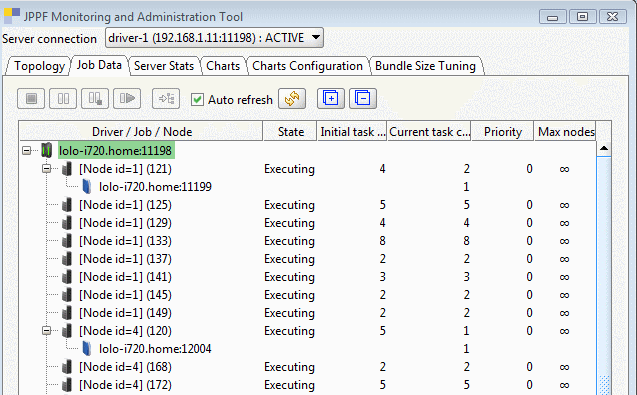
\includegraphics{figures/jppf.png}
      }
      \footnote[frame]{\tiny Picture is from the official site
      http://www.jppf.org}
    \end{column}
  \end{columns}
\end{frame}
